 \section{Architektura}
 Cílem této práce je vytvoření programu, který bude schopen detekovat anomální provoz v IoT sítích. 
 Vzhledem k hardwarovým omezením, které můžou na IoT branách nastat, je architektura navržena tak, aby
 měla co nejmenší nároky na dostupné prostředky. Schéma nasazení detekčního systému se nachází
 na obrázku \ref{obr.deploy-arch}
 
 \begin{figure}[ht]
   \begin{center}
   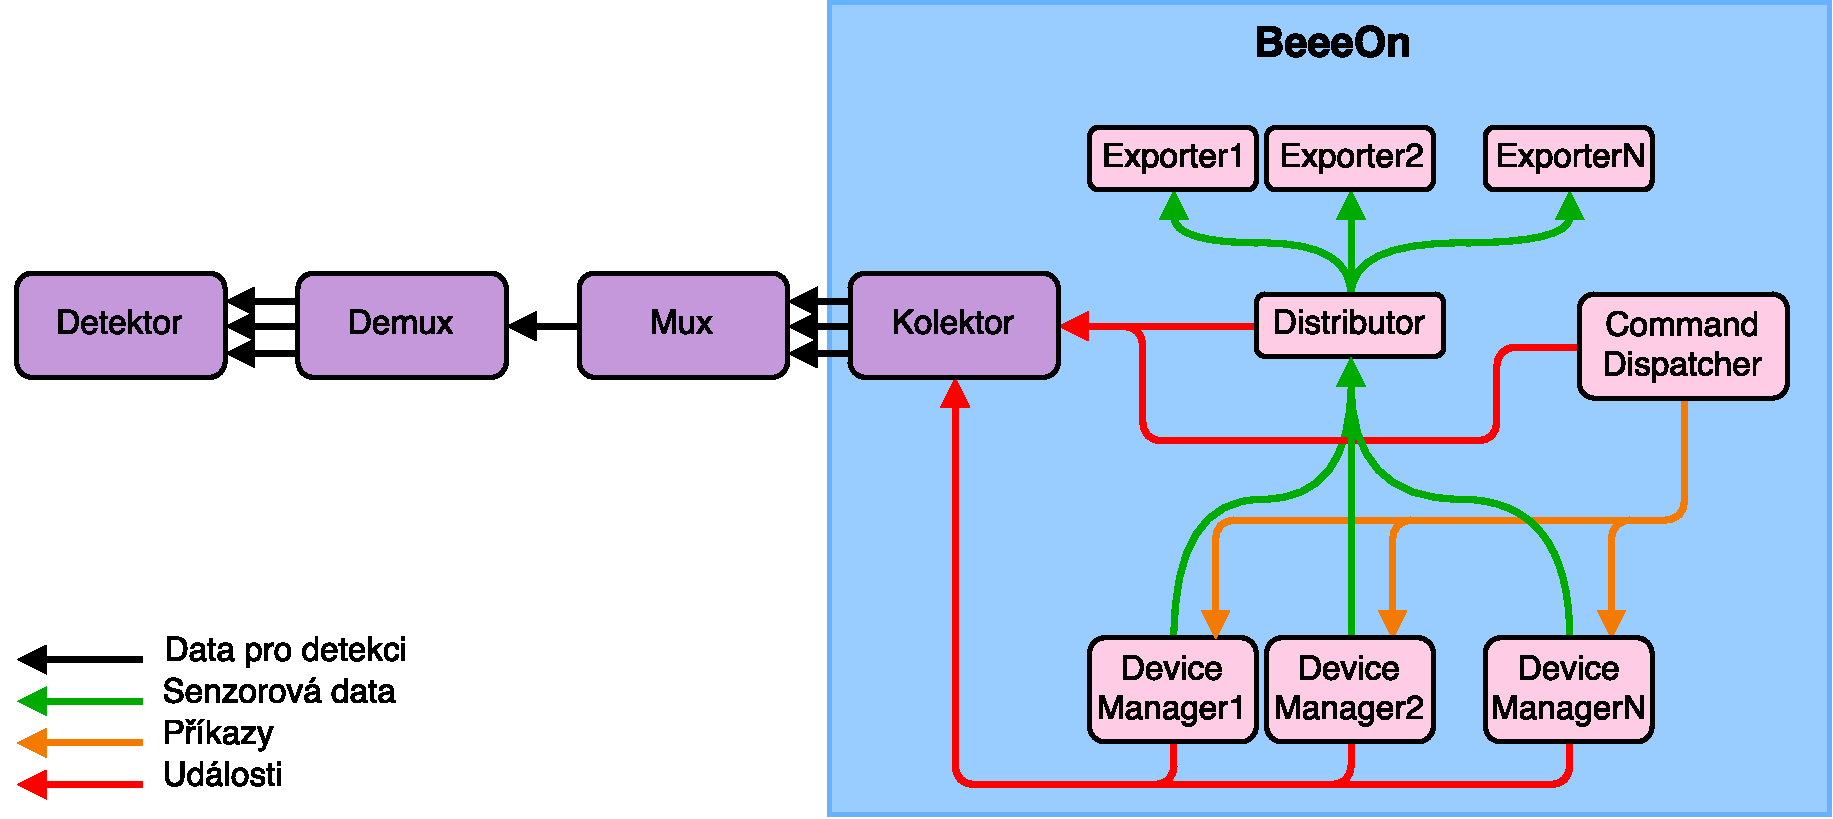
\includegraphics[scale=0.41]{pictures/deploy-arch}
   \caption{Architektura detekčního systému}
   \label{obr.deploy-arch}
   \end{center}
   \end{figure}
 
 Implementace BeeeOn brány obsahuje pro zpracování senzorových dat následující komponenty:
 \begin{itemize}
  \item \textbf{DeviceManager}:
    komponenta definovaná pro každý senzorový protokol, která implementuje veškerou komunikaci
    a zpracování dat
    
  \item \textbf{Distributor}:  
  přijímá data od \textit{DeviceManageru}, která nasledně předává příslušnému \textit{Exporteru}
  
  \item \textbf{Exporter}:
  implementuje protokol, kterým jsou data odesílány z brány
  
  \item \textbf{CommandDispatcher}:  
  komponenta, která přijímá uživatelské příkazy a distribuuje je cílovým komponentám
  
 \end{itemize}
 
 Každá z komponent v BeeeOn bráně navíc využívá návrhový vzor \textit{Observer}, pomocí kterého jsou
 definovány události poskytující informace o každé komponentě. 
 Tímto způsobem bude vytvořený kolektor zíkávat data o provozu, která
 převede do fomátu UniRec (Unified Record) a pomocí systému NEMEA je odešle k analýze.
 
 Exportované informace o provozu bude přijímat detektor, který následně provede jejich zpracování a 
 vyhodnocení stavu. Všechny vytvořené komponety vytvořené pro detekci budou používat rozhraní 
 NEMEA. Díky tomu bude možné komponenty flexibilně provozovat na jednom nebo více různých zařízeních.
 Oddělené nasazení je důležité zejména pro brány s omezenými prostředky, které mohou provádět 
 pouze export dat a o vyhodnocení se bude starat odlišné zařízení s dostatečným výkonem. V případě 
 provozování více bran lze brány používat jako exportéry a veškerá získaná data zpracovávat 
 centrálně. 
 
 Kolektor pro každou událost vytvoří samostnatné výstupní rozhraní. Protože událostí může být 
 velké množství, tak bude vytvořen modul \textit{Mux}, který všechny výstupní rozhraní spojí do jednoho. 
 Pro zpětné rozdělení na jednotlivá rozhraní budou dloužit modul \textit{Demux}. Tyto moduly budou velmi užitečné
 zejména v případě kdy kolektor a detektor budou na rozdílných síťových prvcích, protože údaje 
 o provozu budou přenášeny přes počítačovou síť a bude vyžadováno zabezpeční všech odchozích
 rozhraní. S využítím \textit{Mux} a \textit{Demux} modulů bude stačit zabezpečit pouze jedno sjednocené rozhraní. 
 
 Výhodou návrhu řešení je flexibilita a modularita. Každá komponenta vždy samostatně pokrývá pouze jednu
 část detekčního systému a se díky NEMEA se každá z nich může nacházet na různých síťových prvcích. Zároveň
 v případě potřeby lze vytvořit další moduly, které budou rozšiřovat stávající funcionalitu.
 Podrobnější popis návrhu nově vytvořených komponent detekčního systému se nachází v následujících kapitolách.
 
 \section{Kolektor}
 Úkolem kolektoru bude sběr dostupných dat a jejich odeslání k následné analýze. Informace o 
 provozu budou sbírány z jednotlivých komponent BeeeOn brány, které jsou zpřístupňovány pomocí 
 návrhového vzoru \textit{Observer}. Z tohoto důvodu bude kolektor vždy přímou součástí BeeOn brány. 
 Návrh struktury kolektoru je na obrázku \ref{obr.modelTrid}
 
 \begin{figure}[ht]
   \begin{center}
   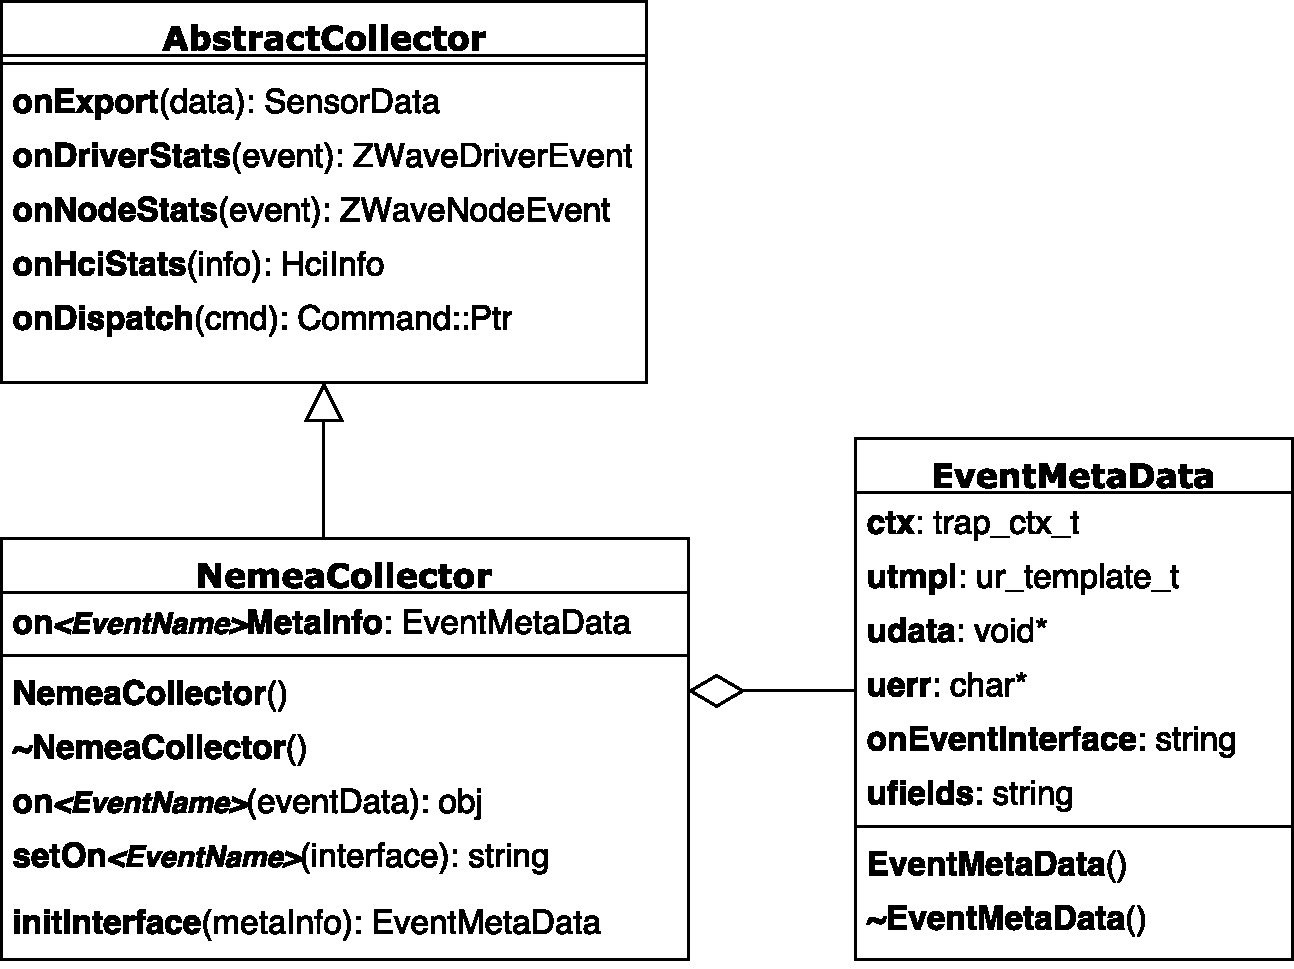
\includegraphics[scale=0.5]{pictures/modelTrid}
   \caption{Návrh kolektoru provozních dat}
   \label{obr.modelTrid}
   \end{center}
   \end{figure}
 
 \textit{AbstractCollector}, je třída vytvořená v projektu BeeeOn, které shromažďuje všechny dostupné události.
 V současné době jsou k dispozici následující události:
 \begin{itemize}
  \item \textbf{onExport}:
   reprezentuje hodnoty dat přicházejících ze senzorů, která jsou odeslána vždy po jejich příjmu
   
  \item \textbf{onDriverStats}:
   v pravidelných intervalech generuje statistiky o Z-Wave sítí dostupné na komunikačních 
   rozhraní
   
  \item \textbf{onNodeStats}:
   periodicky získává informace o jednotlivých prvcích Z-Wava sítě, které jsou dostupné pomocí
   OpenZWave knihovny
   
  \item \textbf{onHciStats}:
   v definovaných intervalech získává z komunikačního rozhraní pro BLE statistiky o provozu
   sítě
  
  \item \textbf{onDispatch}:
  umožňuje získávat zadané uživatelské příkazy
 \end{itemize}

 Vytvořený kolektor bude reprezentován třídou NemeaCollector, která bude potomkem třídy
 \textit{AbstractCollector} a bude implementovat všechny její členské funce pro zachytávání událostí. Pro každou 
 členskou funkci  bude vytvořen setter, který při spuštění brány provede počáteční nastavení
 parametrů pro obsluhu dané 
 události. Vstupním parametrem bude řetězec určující název výstupního rozhraní, který bude
 specifikovaný v 
 konfiguračním souboru BeeeOn brány. Po nastavení počátečních parametrů jako je název výstupního
 rozhraní a seznam UniRec polí se zavolá členská funkce initInterface, jejímž cílem bude inicializace
 veškerých struktur vyžadovaných NEMEA frameworkem.
 Jako vstupní parametr bude přijímán objekt \textit{EventMetaData} udržující veškeré informace potřebné 
 k odesílání získaných dat.
 
 Instace objektu \textit{EventMetaData} bude vytvořena jako členská proměnná třídy \textit{NemeaCollector}
 pro každou členskou funkci události. Díky tomu bude možné každou událost zpracovávat nezávisle dle
 definovaných parametrů.
 
 Definované konstruktory a destuktory budou sloužit jen pro vytvoření a destrukci potřebných 
 struktur. Tímto bude zajištěň programovací idiom RAII (resource acquisition is initialization).
 
 Veškeré odesílané údaje budou rozšířeny o časovou značku a číselný identifikátor, aby mohl detektor
 přesně určit původ případné anomálie.
    
 \section{Detektor}
 Detektor bude hlavní komponentou celého řešení, protože bude vyhodnocovat získaná dat. Vzhledem
 k zadaným požadavkům musí být návrh proveden tak, aby bylo umožněno budoucí rozšiřování. Návrh 
 architektury se nachází na obrázku \ref{obr.detektor}
 \begin{figure}[ht]
   \begin{center}
   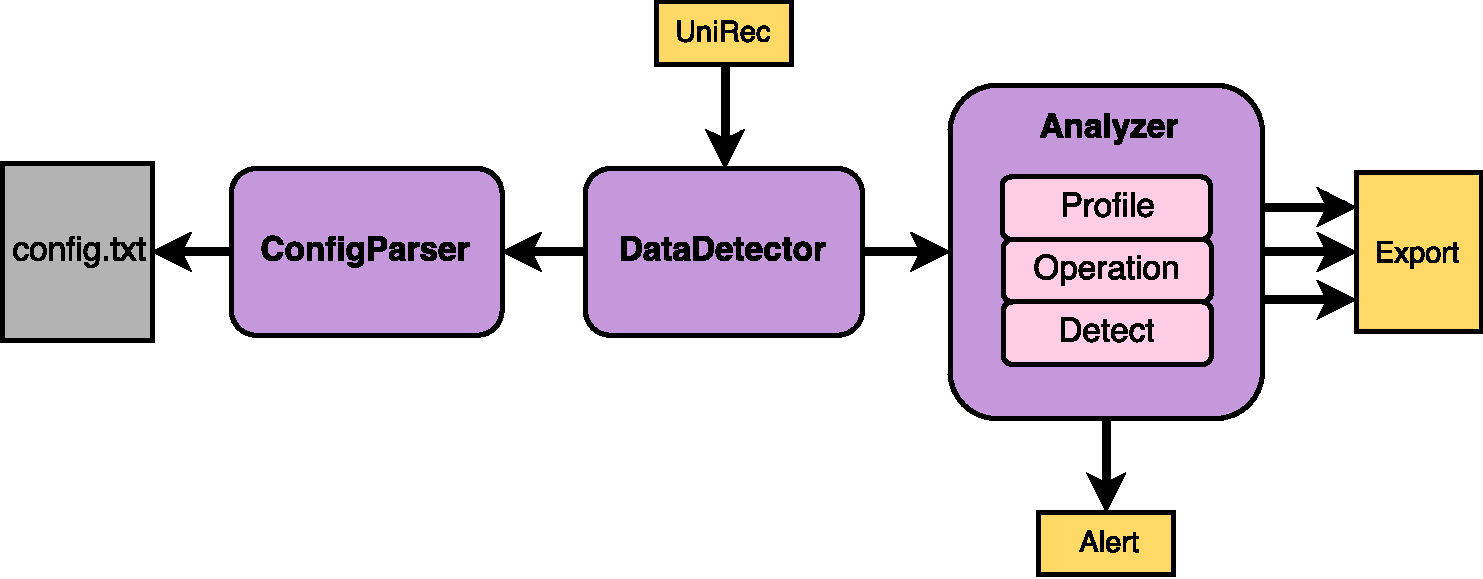
\includegraphics[scale=0.5]{pictures/detektor-arch}
   \caption{Architektura detektoru}
   \label{obr.detektor}
   \end{center}
   \end{figure}

 Komponenta \textit{DataDetector} bude mít jedno vstupní rozhraní, kterým bude přijímat data z kolektoru.
 V případě potřeby
 zpracování více událostí z kolektoru lze využít již existující modul z NEMEA repozitáře, který
 dokáže sloučit více vstupů do jednoho konzolidovaného výstupu. 
 
 Dále se v rámci třídy \textit{DataDetector} bude volat \textit{ConfigParser}, který bude mít na starosti zpracování 
 konfiguračního souboru. Konfigurační soubor bude obsahovat seznam parametrů pro každé UniRec pole,
 na základě kterých bude vytvořena instance třídy \textit{Analyzer} pro analýzu dat. 
 
 Po provedení inicializace všech modulů bude DataDetector pouze přijímat data z kolektoru a 
 předávat je ke zpracování komponentě \textit{Analyzer}. Tato komponenta bude obsahovat
 %!!!!! Sem přidat zmínku o časových řadách.
 tři hlavní části:
 \begin{itemize}
  \item \textbf{Profile}
  
  Bude obsahovat členské funkce, které se budou starat o připravení výchozího profilu sítě. 
  Vytvořený profil bude složen z: průměru, klouzavého průměru, rozptylu a mediánu.
  Tyto hodnoty budou následně použity při porovnávání s aktuálním provozem v rámci detekčních
  metod. V případě potřeby bude možné profil rozšířit o další hodnoty.
  
  \item \textbf{Detect}
  
  Bude sdružovat všechny členské funkce určené pro detekci anomálií v získaných datech. 
  Každá členská funkce bude reprezentovat jedno kritérium a bude možné budoucí rozšíření o další
  potřebné metody.
  
  \item \textbf{Operation}
  
  Cílém této části bude udržování veškerých použitých struktur. Bude se jednat o struktury 
  pro konfiguraci, zpracovávaná data a odesílání získaných výsledků. Odesílat lze informaci o 
  nalezené hrozbě, pro kterou se používá jedno společné rozhraní, nebo lze pravidelně exportovat
  definované části aktuálního profilu sítě pro účelý dalšího zpracování. 
  
 \end{itemize}

 Díky konfiguraci organizované po jednotlivých UniRec polích je možné nastavit chování výše
 popsaných částí nezávisle na sobě pro každé pole.
 
 \subsection{Konfigurace modulu} \label{config_file}
 Jedním z funkčních požadků je možnost konfigurace způsobu detekce, která se tak bude moci přizpůsobit 
 cílovým podmínkám. Každá instance detektoru bude mít jeden konfigurační souboru, který bude 
 popisovat jednotlivá UniRec pole, které se budou analyzovat. 
 
 Konfigurace bude v textové podobě ve formátu klíč a seznam hodnot. Textová podoba je velmi vhodná pro 
 fázi ladění a vývoje nástroje, protože jsou možné manuální úpravy. Cílem ovšem je generovat 
 konfiguraci pomocí externího nástroje, který by mohl být součástí řídící vrstvy IoT brány. Generátor
 nastavení bude velmi vhodný pro koncové uživatele, protože si budou moci přehledně vybrat své
 parametry bez znalosti všech závislotí, které textová konfigurace ani modul pro její zpracování 
 nebude hlídat. Externí nástroj pro definování nastavení analýzy nebude součástí vytvořeného řešení.
 
 Klíčem bude vždy název UniRec pole, které se bude nacházet v příchozích datech. Tento klíč bude 
 oddělen dvojtečnou, za kterou bude sekvence parametrů, které budou odděleny středníkem . Každý klíč
 se bude nacházet na samostatném řádku. Řádky prázdné a začínající znakem \textit{\#} budou
 považovány za komentář. 
 
 
 Definované parametry budou rozděleny do následujících hlavních skupin:
 \begin{itemize}
  \item \textbf{General} 
  
  Tato skupina bude obsahovat obecné volby pro definování časové řady. Pomocí číselných parametrů 
  bude možné určit velikost řady, délku učící fáze, během které je vytvořen profil sítě a její délka
  musí být stejná nebo delší než velikost časové řady, a rozsah ignorovací části, která je vhodná
  k odfiltrování počáteční výměny zprav při navazování spojení. 
  
  Dalším parametrem bude způsob 
  ukládání dat do časové řady. K dispozici budou tři režimy. Prvním z nich bude \textit{simple},
  který přijatou
  hodnotu pouze uloží. Dalším bude \textit{delta}, který bude vkládat pouze rozdíly dvou po
  sobě jdoucích hodnot. 
  Toto je vhodné zejména u časových značek nebo počtu odeslaných zpráv, protože bude vhodnější 
  jednotlivé přírůstky než pouhé absolutní hodnoty. Poslední možností bude \textit{average}, kdy 
  nová příchozí hodnota bude odečtena od aktuálního průměru a výslek bude uložen.
  
  Poslední možností bude číselná hodnota určující rozmezí mezi pravidelnými kontrolami
  přijetí dat a 
  číselný parametr definující periodu pro exportování vybraných parametrů.
  
  \item \textbf{Profile}
  
  Zápis této skupiny je identifikovaný klíčovým slovem \textit{profile}, který má uvnitř kulatých závorek 
  vyjmenované jednotlivé položky, které budou součástí vytvořeného profilu. Ve vytvořeném řešení 
  budou k dispozici následující volby: \textit{average} (průměr), \textit{variance} (rozptyl), 
  \textit{median} (medián) a \textit{cum\_average} (klouzavý průměr).
  
  \item \textbf{Profile Values}
  
  Pro každou položku definovanou v rámci profilu musí být uveden seznam jejich detekčních parametrů.
  Zápis bude probíhat pomocí klíčového slova z profilu, které bude mít jednotlivé hodnoty 
  specifikované uvnitř kulatých závorek. Zde bude možné určit minimální a maximálni soft a hard
  limitých, kterých daná položka aktuálního profilu může dosahovat. Pro soft limit bude možné 
  určit povolenou délku, po kterou může být soft limit překročen (grace period). 
  
  Dalšími parametry budou číselné hodnoty určující hranice pro minimální a maximální velikost 
  změny sledované položky.
  
  Zadání veškerých hodnot nebude nutné a tudíž bude záležet na uživateli, které způsoby detekce 
  bude chtít využít. V případě nedefinování parametru je zapsán znak \textit{-}.
  
  \item \textbf{Export}
  
  Poslední nastavitelnou možností bude export vybraných dat z profilu. Zápis bude probíhat pomocí 
  klíčového slova \textit{export}, který v kulatých závorkách bude mít seznam položek z profilu. Zároveň 
  v případě využití této možnosti bude nutné ve skupině \textit{general} určit časovou periodu
  odesílání.
  Názvy výstupních trap rozhraní
  budou odvozené od klíčů, které se nacházejí před dvojtečkou v konfiguraci.
  %!!! popsat ty posledni dve nuly
  
 \end{itemize}

 Příklad záznamu s konfigurací je na obrázku \ref{obr.config}. Nastavení formou
 souboru bude jedninou volbou pro přizpůsobení detekce. Dále při 
 spuštění programu bude vyžadován jeden přepínač \textit{-i}, který je vyžadován knihovnou trap a 
 bude definovat název vstupního
 rozhraní pro příchozí data a název výstupního rozhraní pro detekované incidenty. 
 
   \begin{figure}[ht]
   \begin{center}
   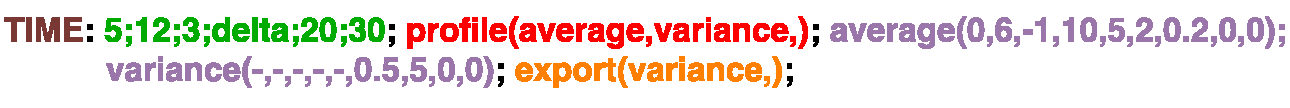
\includegraphics[scale=0.5]{pictures/config-file}
   \caption{Popis konfiguračních parametrů pro jeden záznam}
   \label{obr.config}
   \end{center}
   \end{figure}
 
 \subsection{Použité struktury}
 Velmi důležitou částí návrhu bude určení formátu použitých struktur, které budou urdžovat veškeré 
 údaje nutné pro analýzu. V rámci dektektoru budou potřeba udržovat informace pro následující
 položky:
  \begin{itemize}
   \item \textbf{Konfigurační parametry}
   
   Tato struktura bude hierarchicky ukládat veškeré hodnoty z konfiguračního souboru
   a také údaje nutné k provedení analýzy. V první úrovni se budou nacházet názvy jednotlivých 
   UniRec polí, které budou fungovat jako klíče. V druhé vrstvě se bude nacházet vždy stejná 
   sekvence podklíčů, které budou určovat typ uchovávaných dat. Budou zde uloženy jednotlivé 
   skupiny z konfiguračního souboru \ref{config_file}, které budou označeny stejnojmenými
   identifikátory. Hodnotou těchto skupin budou specifikované parametry detekce dle zapsané
   konfigurace. Dále zde budou podklíče s názvem \textit{metaProfile} a \textit{metaData},
   které budou mít
   stejné hodnoty. Tyto hodnoty budou obsahovat vypočtené údaje z příslušné časové řady
   a zároveň budou umožňovat ukládání dat, která budou nutná k provedení výpočtu 
   a vkládání nových prvků. Rozdíl mezi \textit{metaProfile} a \textit{metaData} bude typ profilu,
   pro který budou určeny. Podklíč \textit{metaProfile} bude uchovávat údaje pro základní profil,
   který bude vytvořen během učící fáze a bude sloužit pro určení anomálie. Zatímco 
   hodnoty v \textit{metaData} budou vztaženy k aktuálnímu profilu sítě, který se mění s každým
   nový prvkem v časové řadě.
   
   \item \textbf{Senzorová data}
   
   Cílem této struktury bude hierarchicky ukládat přicházející data z kolektoru do časových řad. 
   V první úrovni se jako v předchozím případě budou nacházet názvy jednotlivých UniRec polí. 
   Protože jedno UniRec pole může reprezentovat data z více různých senzorů nebo bran, tak se na 
   další úrovni nachází identifikátor zdroje dat. Předpokládá se, že každá použitá brána a senzor 
   má v rámci jedné instance detektoru unikatní identifikátory. Na třetí úrovni se již vyskytuje 
   definovaná časová, která ukládá data podle zadané konfigurace.
   
   \item \textbf{Nastavení pro export} 
  \end{itemize}

 
 
 \subsection{Způsob analýzy}
 popis analýzy
  stavový diagram zpracování
  soft hard limit, data change, .... 
  časové řady
  
 \section{Multiplexor a demultiplexor}
 
 \section{Scénáře útoků}
  Odvození na základě experimentů a analýzy